\documentclass{beamer}
\usepackage{amsfonts}
\usepackage{amsmath}
\usepackage{/Users/timbarry/optionFiles/mymacros}
%Information to be included in the title page:
\title{A generalized errors-in-variables model, with application to single-cell CRISPR screens}
\author{Tim Barry$^1$, Eugene Katsevich$^2$, Kathyrn Roeder$^1$}
\institute{$^1$CMU Statistics and Data Science\\ $^2$Wharton Statistics and Data Science}
\date{September 2021}
\DeclareMathOperator*{\argmin}{arg\,min}

\begin{document}
	
\frame{\titlepage}
	
\begin{frame}
\frametitle{Overview}
\begin{itemize}
\item \textbf{Background}
\item Analysis objective and challenges
\item Existing approach
\item Proposed method
\item Simulation results
\item Real data results
\end{itemize}
\end{frame}
	
\begin{frame}
\frametitle{Single-cell CRISPR screens are a powerful technology for mapping the regulatory wiring of the genome.}

\begin{figure}
	\centering
	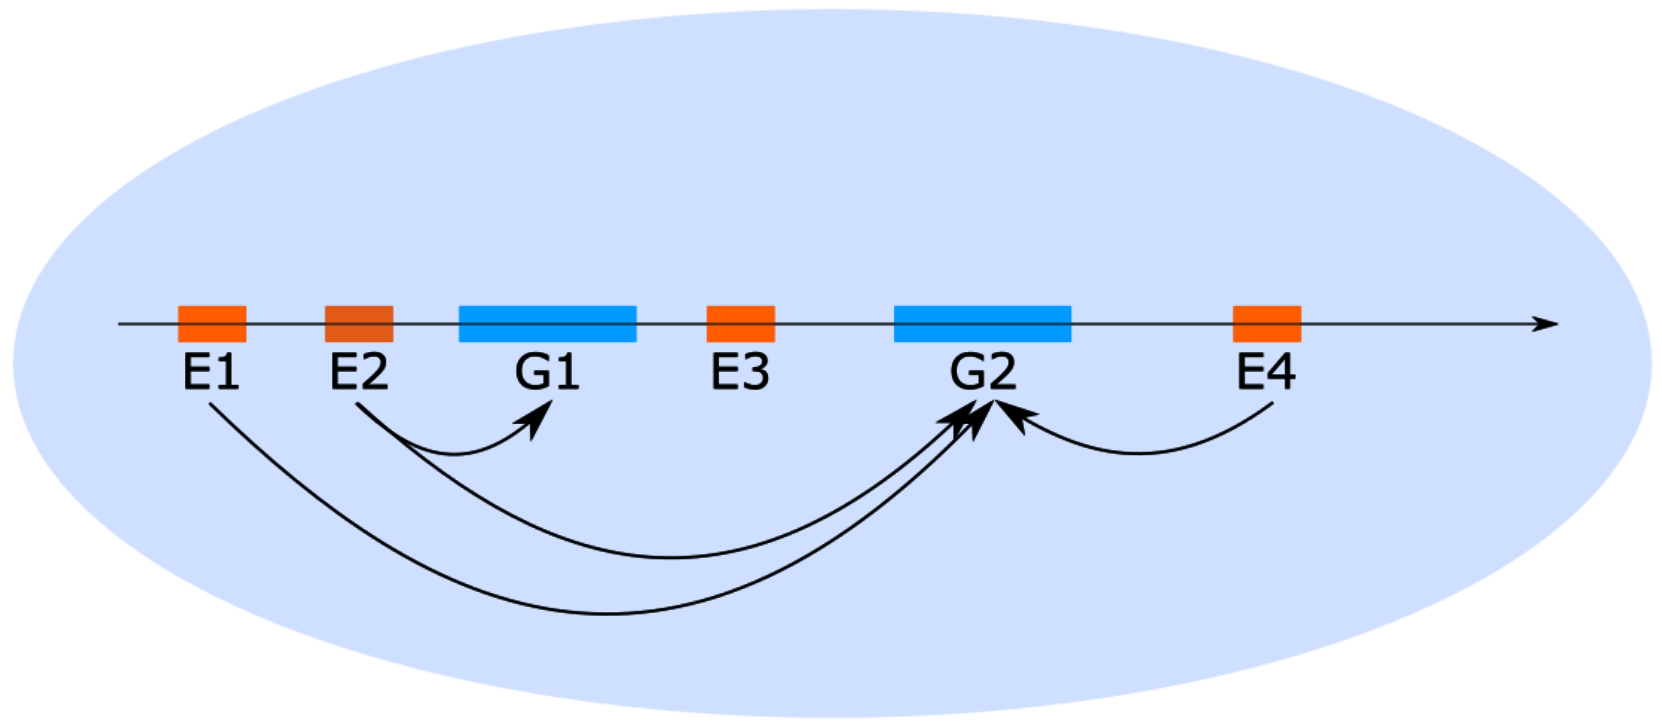
\includegraphics[width=1\linewidth]{extra_figs/regulatory_wiring}
	\label{regulatorywiring}
\end{figure}
\end{frame}
	
\begin{frame}
	\frametitle{Single-cell CRISPR screens entail sequencing gRNAs and mRNAs in individual cells.}
	\begin{figure}
		\centering
		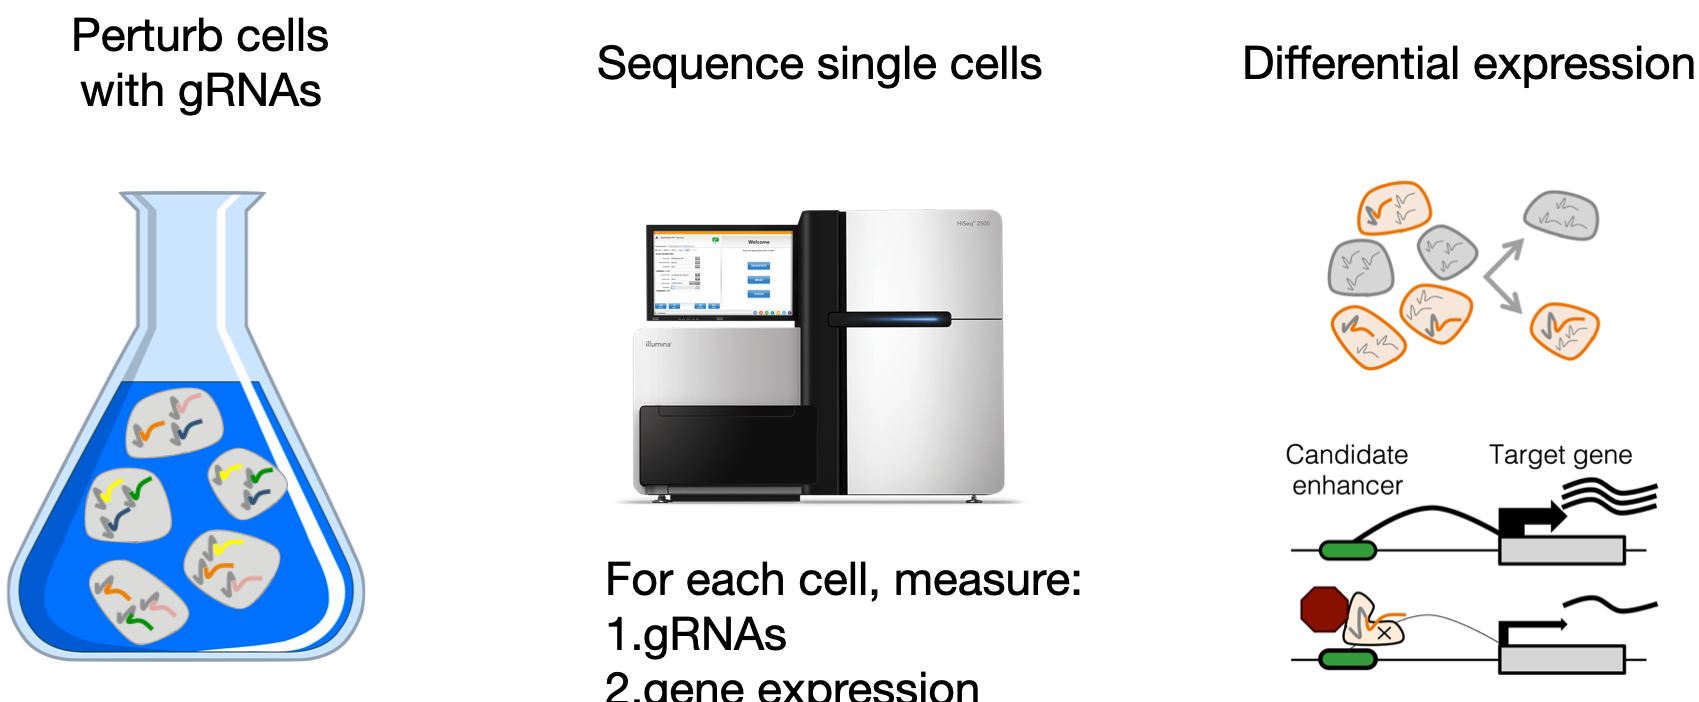
\includegraphics[width=1\linewidth]{extra_figs/experimental_protocol}
	\end{figure}
\end{frame}

\begin{frame}
\frametitle{We investigate single-cell CRISPR screen datasets produced by \cite{Gasperini2019} and \cite{Xie2019}.}
\begin{figure}
	\centering
	
\includegraphics[width=1.0\linewidth]{extra_figs/papers}
\end{figure}
\end{frame}


\begin{frame}
\frametitle{Overview}
\begin{itemize}
	\item Background
	\item\textbf{Analysis Challenges}
	\item Existing approach
	\item Proposed method
	\item Simulation results
	\item Real data results
\end{itemize}
\end{frame}

\begin{frame}
\frametitle{There are several challenges to the analysis of single-cell CRISPR screen data:}

\begin{itemize}
\item[1.] The perturbation is unobserved.
\item[2.] Technical factors, such as batch and sequencing depth, explain variability in mRNA and gRNA counts.
\item[3.] Unperturbed cells exhibit ``background gRNA reads.'' \cite{Schraivogel2020}
\item[4.] The mRNA and gRNA expression data are highly discrete.
\end{itemize}
\end{frame}

\begin{frame}
\frametitle{(1) The perturbation is unobserved, and (2) technical factors are present.}
\begin{figure}
	\centering
	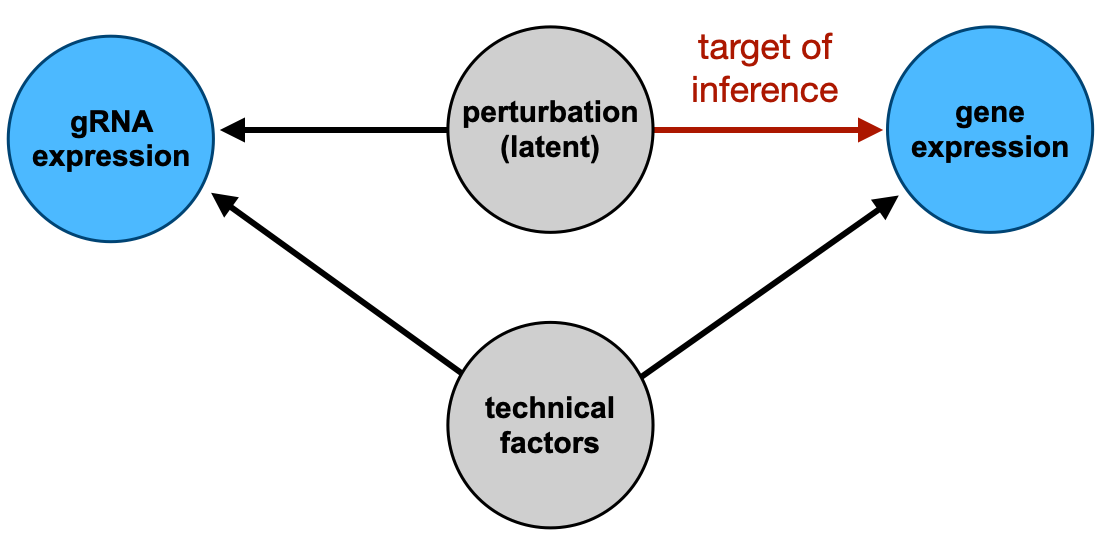
\includegraphics[width=1\linewidth]{../figures/fig1/dag}
	\label{dag}
\end{figure}
\end{frame}

\begin{frame}
\frametitle{(3) Unperturbed cells exhibit background gRNA reads.}
\begin{figure}
	\centering
	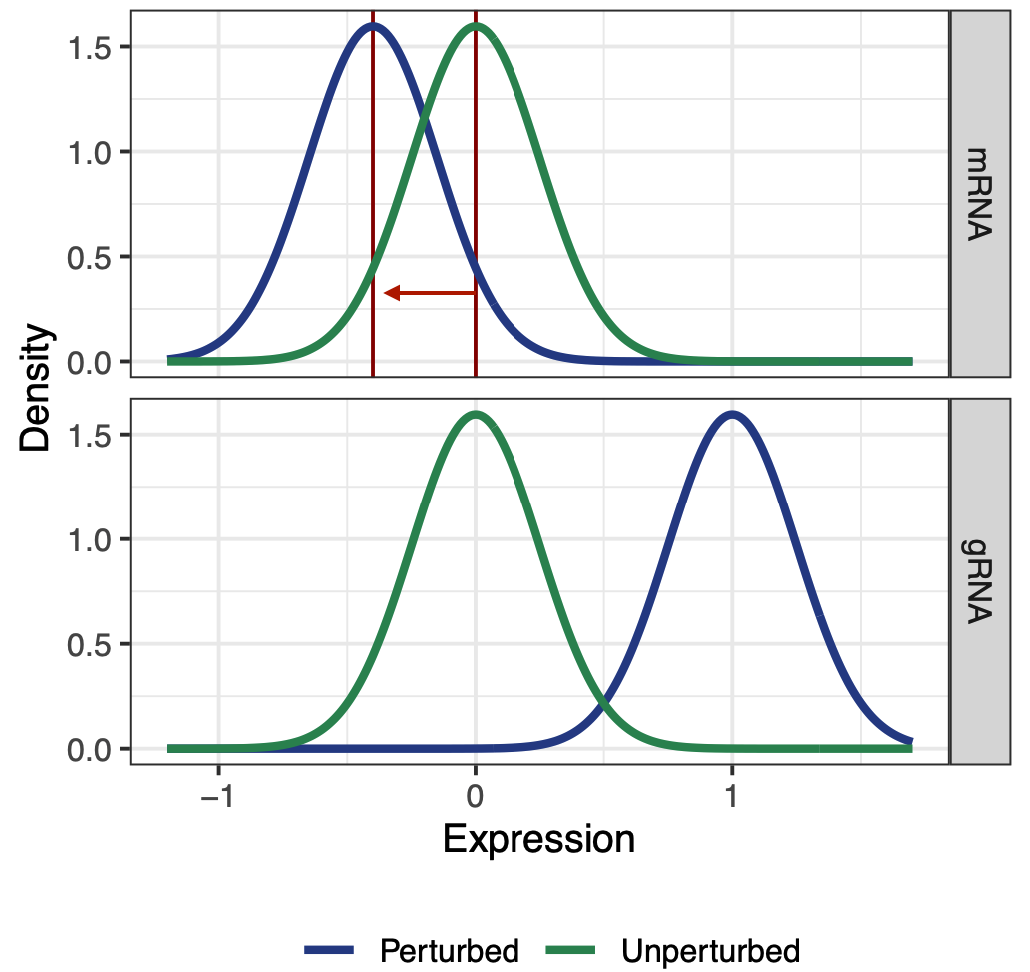
\includegraphics[width=0.75\linewidth]{../figures/fig1/density_plot_annotated.png}
\end{figure}
\end{frame}


\begin{frame}
\frametitle{(4) The count data are highly discrete.}
\begin{figure}
	\centering
	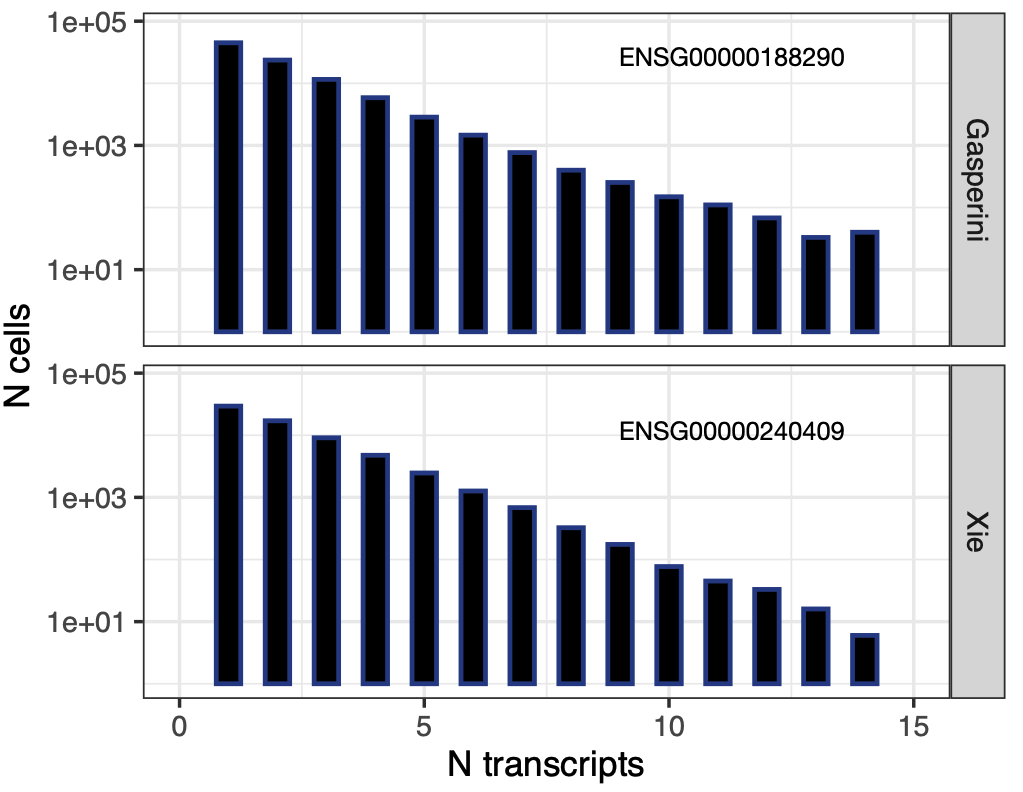
\includegraphics[width=0.75\linewidth]{../figures/fig1/mRNA_count_hist_annotated.png}
\end{figure}
\end{frame}


\begin{frame}
\frametitle{Overview}
\begin{itemize}
	\item Background
	\item Analysis Challenges
	\item \textbf{Existing approach}
	\item Proposed method
	\item Simulation results
	\item Real data results
\end{itemize}
\end{frame}


\begin{frame}
\frametitle{Data and notation}

\begin{itemize}
\item Observe $n \approx 100,000 - 250,000$ cells.
\item Consider a given mRNA and gRNA of interest.
\item For cell $i \in \{1, \dots, n\}$, let 
\begin{itemize}
\item $p_i \in \{0, 1\}$ indicate whether a perturbation occurred. 
\item $m_i \in \mathbb{N}$ be the mRNA count.
\item $g_i \in \mathbb{N}$ be the gRNA count.
\item $l^m_i \in \mathbb{N}$ be the mRNA library size.
\item $z_i \in \R^{d-1}$ be a vector of technical factors, possibly including an intercept term.
\end{itemize}
\item We measure $\approx5,000$ genes, $\approx500 - 5,000$ gRNAs
\end{itemize}
\end{frame}

\begin{frame}
\frametitle{The ``thresholding method''}

\begin{itemize}
\item[1.] For given threshold $c \in \N$, estimate $p_i$ by $$ \begin{cases} \hat{p}_i = 0 \textrm{ if } g_i \geq c, \\ \hat{p}_i = 1 \textrm{ if } g_i < c \end{cases}.$$
\item[2.] Fit the regression model \cite{Sarkar2021}
$$ m_i | \left( z_i, l^m_i \right) \sim \textrm{NB}_\theta(\mu_i),$$ where $\theta >0$ is the NB size parameter, and $$\log\left(\mu_i\right) = \beta_m \hat{p}_i + \gamma^T_m z_i + \log\left( l_i^m\right).$$
\item[3.] Obtain an estimate $\hat{\beta}_m$ of $\beta_m$ and compute a CI for $\beta_m$.
\end{itemize}
\end{frame}

\begin{frame}
\frametitle{Problem 1: There is no clear location in the data at which to draw the threshold.}
\begin{figure}
	\centering
	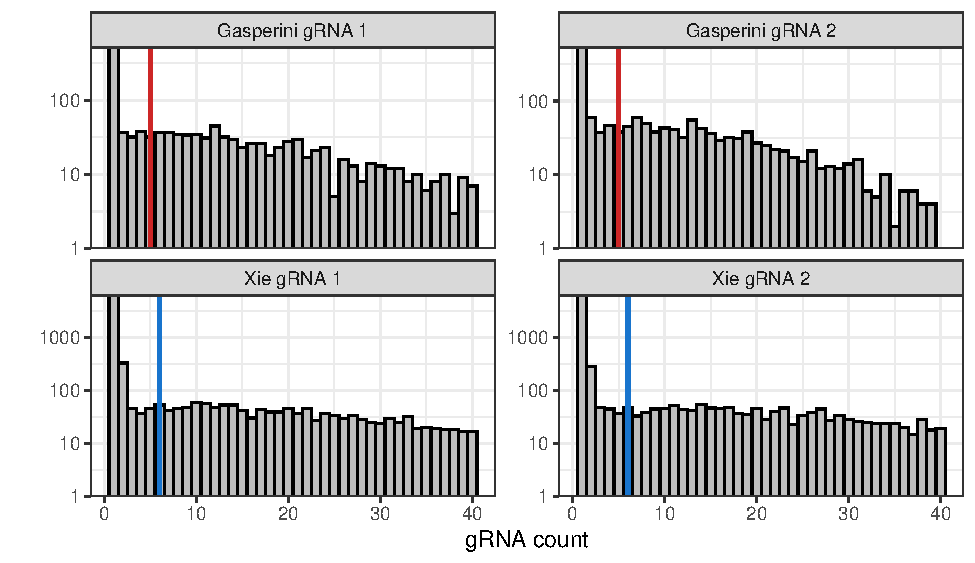
\includegraphics[width=1\linewidth]{../figures/fig2/histograms}
\end{figure}


\end{frame}


\begin{frame}
\frametitle{Problem 2: Thresholding can lead to attenuation bias.}


As a simple example, suppose
$$
\begin{cases}
p_1, \dots, p_n \sim \textrm{Bern}(\pi) \\
y_i = \beta_m p_i + \ep_i \\
x_i = \beta_g p_i + \tau_i,
\end{cases}
$$
where $\ep_i \indep \tau_i$ and $\ep_i, \tau_i \sim N(0,1)$. We observe
$$ \{(x_1, y_1), \dots, (x_n, y_n)\},$$ and we want to estimate $\beta_m$ using the thresholding method. Assume $\beta_g$ and $\pi$ are known. We select the threshold $c$ so as to minimize the misclassification rate, i.e., $$c = \argmin_{c \in \R} \frac{1}{n} \sum_{i=1}^n \mathbb{I}(\hat{p}_i \neq p_i).$$

\end{frame}


\begin{frame}
\frametitle{The thresholding method shows clear attenuation bias.}
\begin{itemize}
\item We set $\beta_m$ to 1.
\end{itemize}

\begin{figure}
	\centering
	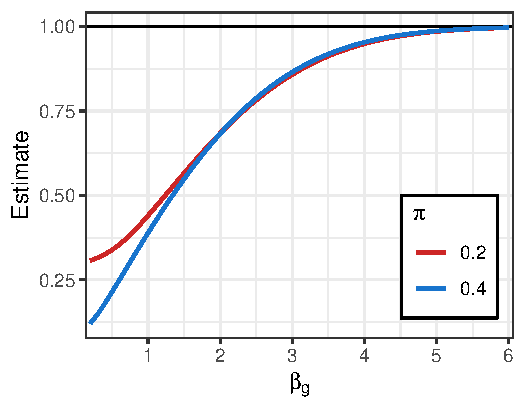
\includegraphics[width=0.75\linewidth]{../figures/fig2/att_bias}
\end{figure}


\end{frame}

\begin{frame}
\frametitle{Research question}
Does modeling the gRNA count distribution (thereby bypassing thresholding) improve estimation and inference?
\end{frame}


\begin{frame}
\frametitle{Overview}
\begin{itemize}
	\item Background
	\item Analysis Challenges
	\item Existing approach
	\item \textbf{Proposed method}
	\item Simulation results
	\item Real data results
\end{itemize}
\end{frame}


\begin{frame}
\frametitle{A bit more notation}
For cell $i \in \{ 1, \dots, n\}$, let $l^g_i$ be the gRNA library size.
\end{frame}

\begin{frame}
\frametitle{We extend the parametric model of \cite{Sarkar2021} to model both mRNA \textit{and} gRNA counts.}
\begin{itemize}
\item[1.] \textbf{mRNA}: $m_i | (z_i, l_i^m) \sim \textrm{NB}_\theta(\mu^m_i),$ where $$ \log\left( \mu^m_i \right) = \beta_m p_i + \gamma_m^T z_i + \log(l^m_i).$$
\item[2.] \textbf{gRNA}: $g_i | (z_i, l_i^g) \sim \textrm{NB}_\theta (\mu_i^g),$ where $$\log(\mu_i^g) = \beta_g p_i + \gamma_g^T z_i + \log(l_i^g)$$
\item[3.] \textbf{Perturbation}: $p_i \sim \textrm{Bern}(\pi)$, where $\pi \in [0, 1/2)$. $p_i$ is latent.
\end{itemize}
\end{frame}

\begin{frame}
\frametitle{Generalizing the NB model to arbitrary exponential family response distribution and link function yields the ``GLM-EIV'' (GLM errors-in-variables) model.}

This extension is important, because authors have used
 \begin{itemize}
 \item \textcolor{blue}{Negative binomial}, \cite{Choudhary2021}
 \item \textcolor{blue}{Poisson}, \cite{Schraivogel2020}
 \item and \textcolor{blue}{Gaussian} \cite{Lin2021}
 \end{itemize}
distributions to model single-cell data.
\end{frame}


\begin{frame}
\frametitle{Generalizing the NB model to arbitrary exponential family response distribution and link function yields the ``GLM-EIV'' (GLM errors-in-variables) model.}

\begin{itemize}
\item[1.] \textbf{mRNA density}: $$f_m(m_i; \eta^m_i) = \exp\left\{m_i \eta_i^m - \psi_m(\eta_i^m) + c_m(m_i) \right\}.$$
\item[2.] \textbf{gRNA density}: $$f_g(g_i; \eta^g_i) = \exp\left\{ g_i \eta_i^g - \psi_g(\eta_i^g) + c_g(g_i) \right\}.$$
\item[3.] \textbf{Perturbation density}: $$ f(p_i) = \pi^{p_i} (1-\pi)^{1-p_i}.$$
\end{itemize}
\end{frame}

\begin{frame}
\frametitle{Generalizing the NB model to arbitrary exponential family response distribution and link function yields the ``GLM-EIV'' (GLM errors-in-variables) model.}

Consider the mRNA model.
\begin{itemize}
\item Let $g_m : \R \to \R$ be the link function, i.e.
$$g_m(\mu_i) = \beta_m p_i + \gamma^T_m z_i + \log(l_i^m).$$
\item The canonical parameter for the $i$th cell, $\eta^m_i$, is given by
$$ \eta_i^m = \left[ \psi_m' \right]^{-1} \left( \mu_i \right) = \left[ \psi'_m \right]^{-1} \left( g_m^{-1} \left( \beta_m p_i + \gamma_m^T z_i + \log(l_i^m) \right)\right).$$
\item Thus, the model is defined by (i) the cumulant-generating function $\psi_m$, and (ii) the link function $g_m$. 
\end{itemize}
\end{frame}

\begin{frame}
\frametitle{We derive an EM algorithm to fit the model.}
\textbf{E step}:
\begin{itemize}
\item Compute membership probabilities $T_1, \dots, T_n$ using the model.
\end{itemize}

\textbf{M step}:
\begin{itemize}
\item Augment count vectors $m \rightarrow [m, m], g \rightarrow [g, g]$.
\item Augment offset vectors $l_m \rightarrow [l_m, l_m], l_g \rightarrow [l_g, l_g]$.
\item Augment covariate matrix  $Z \rightarrow [Z, Z];$ append column of $1$s and $0$s for perturbation indicators.
\item Fit weighted GLM to both modalities using membership probabilities $[T_1, \dots, T_n, 1 - T_1, \dots, 1 - T_n]$ as weights.
\end{itemize}
\end{frame}


\begin{frame}
\frametitle{We use statistical tricks to produce an accurate pilot estimate of the parameters, enabling us to run the EM algorithm using only one restart.}
\begin{itemize}
	\item Naive approach (random parameter initialization): $$\left( \textrm{15 EM restarts} \right) \left( \frac{ \textrm{20 iterations} }{\textrm{EM restart}} \right) \left( \frac{\textrm{2 GLMs}}{\textrm{iteration}}\right) \approx \textrm{600 GLMs}.$$
	\item GLM-EIV approach: 
	$$ \left(\textrm{1 EM restart}\right) \left( \frac{ \textrm{3 iterations}}{\textrm{EM restart}} \right)\left( \frac{ \textrm{2 GLMs} }{ \textrm{iteration} } \right) \approx \textrm{6 GLMs}.$$
\end{itemize}
\end{frame}


\begin{frame}
\frametitle{We derive an analytic expression for the observed information matrix to enable fast inference (CIs, $p$-values).}
\begin{multline*}
J(\hat{\theta}; m, g) = -\E \left[\nabla^2 \mathcal{L}(\theta; m, g, p) | g, m, \hat{\theta} \right] \\ + \E\left[ \nabla \mathcal{L}(\theta; m, g, p) |  g, m, \hat{\theta} \right] \E\left[ \nabla \mathcal{L}(\theta; m, g, p) | g, m, \hat{\theta}\right]^T \\ - \E\left[ \nabla\mathcal{L}(\theta; m, g, p) \nabla \mathcal{L}(\theta; m, g, p)^T | g, m, \hat{\theta} \right].
\end{multline*}
\end{frame}

\begin{frame}
\frametitle{We develop a pipeline to deploy the method across hundreds or thousands of processors on HPC and cloud.}

\begin{figure}
	\centering
	
\includegraphics[width=0.6\linewidth]{extra_figs/computing}
\end{figure}
\end{frame}

\begin{frame}
\frametitle{Method summary}
\begin{itemize}
\item We extend the parametric model of \cite{Sarkar2021} to model both mRNA counts and gRNA counts.
\begin{itemize}
\item Arbitrary exponential family distributions and link functions are supported. 
\end{itemize}
\item We (i) propose a fast EM algorithm to fit the model, (ii) derive an analytic expression for the observed information matrix, and (iii) implement a computational pipeline to deploy the method on HPC and cloud. 
\begin{itemize}
\item These features enable GLM-EIV to scale to large datasets.
\end{itemize}
\end{itemize}
\end{frame}

\begin{frame}
\frametitle{Overview}
\begin{itemize}
	\item Background
	\item Analysis objective and challenges
	\item Existing approach
	\item Proposed method
	\item \textbf{Simulation results}
	\item Real data results
\end{itemize}
\end{frame}

\begin{frame}
\frametitle{Simulation setup}
\begin{itemize}
\item No covariates
\item No offset terms (i.e., library size fixed at one)
\item Intercept terms fixed
\item $\pi$ fixed
\item $\beta_m$ fixed (and of moderate size)
\item $\beta_g$ varied over an interval
\item Gaussian, Poisson, and negative binomial distributions
\end{itemize}
\end{frame}

\begin{frame}
\begin{figure}
	\centering
	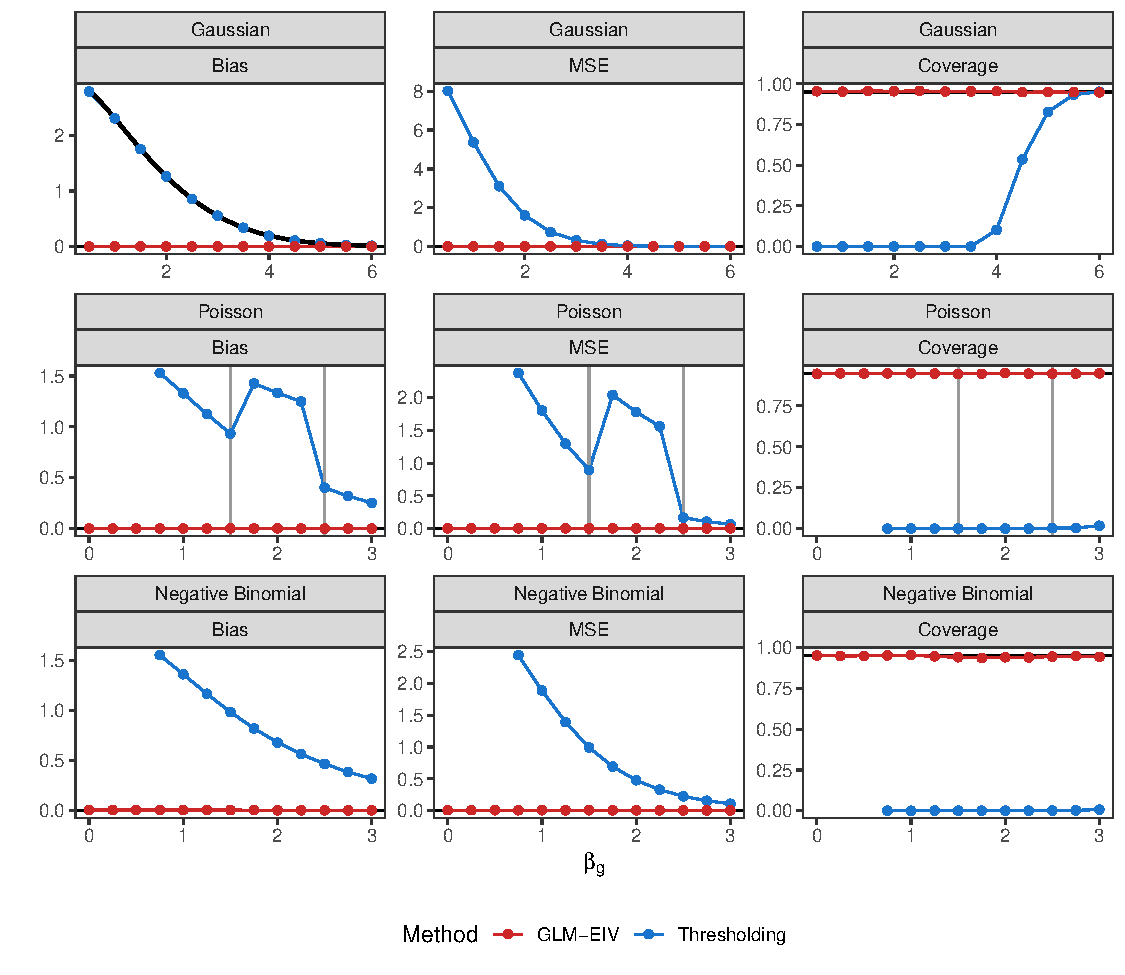
\includegraphics[width=1\linewidth]{../figures/fig3/simulation_warmup_arm_g}
\end{figure}
\end{frame}


\begin{frame}
\frametitle{GLM-EIV outperforms the thresholding method on the simulated data for two main reasons:}
\begin{itemize}
\item[1.] GLM-EIV leverages information from \textit{both} modalities to assign perturbation identities to cells.
\item[2.] GLM-EIV generates \textit{soft} rather than \textit{hard} assignments, capturing the inherent uncertainty in whether a perturbation occurred.
\end{itemize}
\end{frame}

\begin{frame}
\frametitle{Overview}
\begin{itemize}
	\item Background
	\item Analysis objective and challenges
	\item Existing approach
	\item Proposed method
	\item Simulation results
	\item\textbf{Real data results}
\end{itemize}
\end{frame}


\begin{frame}
\frametitle{We followed recommendations of \cite{Choudhary2021} for quality control and modeling.}

\begin{itemize}
\item Quality control
\begin{itemize}
\item Lowly-expressed genes filtered
\item Cells with library sizes below 5th percentile or above 95th percentile filtered
\end{itemize}
\item mRNA model
\begin{itemize}
\item used negative binomial distribution (with log link)
\item size parameter $\theta$ estimated from data
\end{itemize}
\item gRNA model
\begin{itemize}
\item used Poisson distribution (with log link)
\end{itemize}
\end{itemize}
\end{frame}


\begin{frame}
\frametitle{The estimate $\hat{\beta}_g$ for $\beta_g$ was large on both datasets across all site types.}
\begin{center}
\textbf{Gasperini}
\end{center}
\begin{center}
\begin{tabular}{|c|c|}
	\hline 
	Site type & Mean $\exp\left(\beta_g\right)$ 95\% CI \\ 
	\hline 
 	 \textcolor{blue}{Candidate \textit{cis}} & $(4453, 5353)$ \\ 
	\hline 
	\textcolor{blue}{Negative control} &  $(4484, 5408)$ \\ 
	\hline
	\textcolor{blue}{TSS-targeting} & $(3605, 4205)$ \\
	\hline
\end{tabular} 
\end{center}

\begin{center}
	\textbf{Xie}
\end{center}
\begin{center}
	\begin{tabular}{|c|c|}
		\hline 
		Site type & Mean $\exp\left(\beta_g\right)$ 95\% CI \\ 
		\hline 
		\textcolor{blue}{Candidate \textit{cis}} & $(307, 324)$ \\ 
		\hline 
		\textcolor{blue}{Negative control} &  $(299, 316)$ \\
		\hline
	\end{tabular} 
\end{center}



\end{frame}


\begin{frame}
\frametitle{GLM-EIV and thresholding exhibited similar CI coverage rates on the negative control pairs.}
\begin{center}
\begin{tabular}{|c|c|c|}
	\hline 
	Dataset & GLM-EIV & Thresholding \\ 
	\hline 
	\textcolor{blue}{Xie} & 93.7\% & 93.2\% \\ 
	\hline 
	\textcolor{blue}{Gasperini} & 90.6\% & 91.4\%  \\ 
	\hline 
\end{tabular}
\end{center}
\end{frame}


\begin{frame}
\frametitle{Estimates and CIs produced by GLM-EIV and the thresholding method were similar.}
\begin{figure}
	\centering
	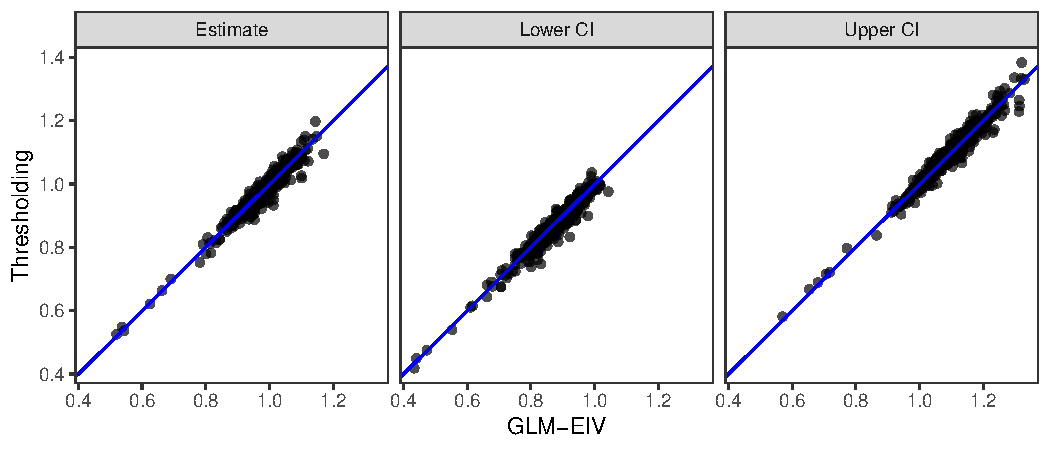
\includegraphics[width=1\linewidth]{../figures/fig5/comparison}
\end{figure}
\begin{center}
Candidate \textit{cis} pairs in Xie et al.\ data.
\end{center}
\end{frame}

\begin{frame}
\frametitle{We now can answer our core research question.}
\textbf{Research question}: Does modeling the gRNA count distribution (thereby bypassing thresholding) improve estimation and inference?
\begin{itemize}
\item Yes, if the problem is in a ``sufficiently challenging'' setting.
\item The real data that we analyzed, surprisingly, were in an ``easy'' setting.
\item Therefore, GLM-EIV and the thresholding method performed similarly on the real data.
\end{itemize}
\end{frame}


\begin{frame}
\frametitle{The proposed method could help solve practical challenges.}
\begin{itemize}
\item Selecting cell-specific thresholds
\item Identifying ``problem difficulty'' and thus whether thresholding is appropriate
\end{itemize}
\end{frame}

\begin{frame}
\frametitle{Together, GLM-EIV and SCEPTRE shed light on core analysis challenges posed by single-cell CRISPR screens, paving the way for the development of new methods.}
\begin{itemize}
	\item[1.] Perturbation unobserved
	\item[2.] Confounders and nuisance variables
	\item[3.] Possible model mispecification
	\item[4.] Background reads
	\item[5.] Highly discrete data
	\item[6.] Ineffective gRNAs
\end{itemize}
\end{frame}

\begin{frame}
\frametitle{Thank you.}
Acknowledgments:
\begin{itemize}
\item Xuran Wang helped with the Xie data preprocessing.
\item All analyses were run on Pittsburgh Supercomputer.
\end{itemize}
\end{frame}

% However, the model gives us many insights into single-cell CRISPR screen datasets.
% What is the fold change in gRNA expression?
% What is the perturbation probability?
% Practical strategies:
% Is thresholding a reasonable strategy for these data?
% How can I choose a good threshold (cell-specific threshold; use only cells with high or low posterior membership probabilities, and throw all others out)?

\bibliography{/Users/timbarry/optionFiles/glmeiv.bib}
\bibliographystyle{apalike}

\end{document}
